\section{Number theory}


\begin{definition*}


  \defn{prime factorization}
  \begin{mdframed}
    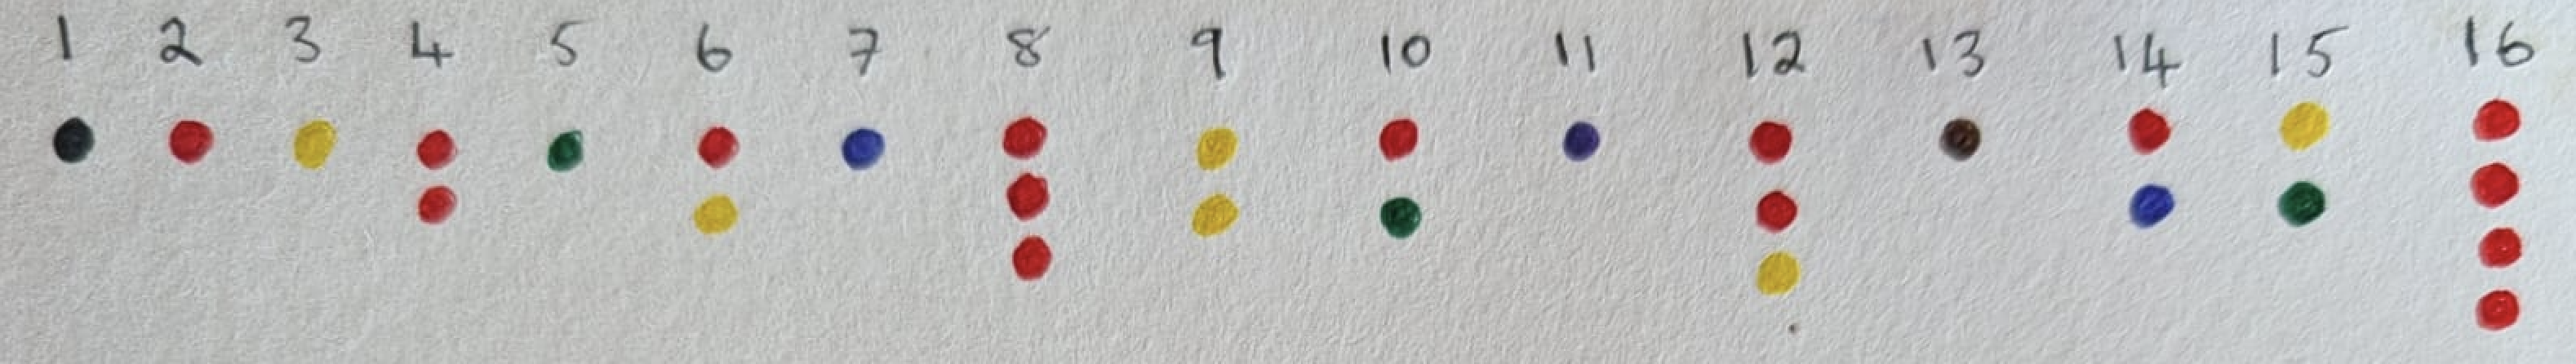
\includegraphics[width=400pt]{img/foundations--integers-e251.png}
  \end{mdframed}

 $c | a$, i.e. $c$ \defn{divides} $a$ ($a$ is a \defn{multiple} of $c$), i.e. if there exists $d$ such that $cd = a$.

 $\gcd(a, b)$, the \defn{greatest common divisor} of $a$ and $b$, is the largest integer $c$ such that $c | a$ and $c | b$.

  $a$ and $b$ are \defn{relatively prime} aka \defn{coprime} if $\gcd(a, b) = 1$.

  $\lcm(c, d)$ is the smallest integer $a$ such that $c|a$ and $d|a$.
\end{definition*}

  Question: why exactly are we contemplating products here, as opposed to e.g. sums?




\begin{remark*}
  a \defn{multiple} of a prime is a number whose factorization contains that prime.

  $c$ \defn{divides} $a$ ($a$ is a \defn{multiple} of $c$) if $a$'s factorization is a ``multiplicity superset​'' of $c$'s.

  The $\gcd$ is the largest integer whose factorization is a ``subset​'' of both factorizations.

  If $a$ and $b$ are relatively prime then their factorizations have no overlap.

  The $\lcm$ is the smallest integer whose factorization is a ``superset​'' of both factorizations.

  If $a$ is a multiple of $c$ then their $\lcm$ is $a$.

  If $a$ and $b$ are relatively prime then their $\lcm$ is their product.
\end{remark*}

\begin{example*}
Consider $2^2 \cdot 3 = 12$ and $2\cdot 3^2 = 18$.

Their factorizations have much in common (they are certainly not coprime), but neither is a
multiple of the other.

Their $\lcm$ is the first number that is a ``multiplicity superset​'' of the other: i.e. we must add
a factor of $3$ to $12$'s factorization, or an additional $2$ to $18$'s, either way
yielding $2^2 \cdot 3^2 = 36$.

Note that their $\lcm$ is not one of them (as it would be if one divided the other), but it is
smaller than their product.

The $\gcd$ of $2^2\cdot 3$ and $2\cdot 3^2$ is $2\cdot 3$.
\end{example*}


\begin{example*}
    For example if
  \begin{align*}
    a = 12 &= 2^2 \cdot 3 \\
    b = 40 &= 2^3 \cdot 5 \\
  \end{align*}
  then $\gcd(a, b) = 2^2 = 4$ and $\lcm(a, b) = 2^3 \cdot 3 \cdot 5 = 120$.

  This can be written as a general theorem involving mins and maxes in the exponents of a product
  of primes.
\end{example*}


\begin{theorem*}
  $\gcd(a,b) \times \lcm(a,b) = ab$
\end{theorem*}

\begin{example*}
  The product of  $2^2\cdot 3$ and $2\cdot 3^2$ is their concatenation: $2^2 \cdot 3 \cdot 2 \cdot 3^2 = 12 \cdot 18 = 216$.

  This is the product of their $\gcd$ $2\cdot 3$ and their $\lcm$ $2^2\cdot 3^2$.
\end{example*}


\begin{intuition*}
  We're performing additive operations on the exponents of the prime factors. The product is the
  sum of all; the $\gcd$ takes the min from each and is thus missing the maxes; the $\lcm$ takes
  the max from each and is thus missing the mins; their product contains the full multiplicities of
  all factors.
\end{intuition*}


\begin{mdframed}
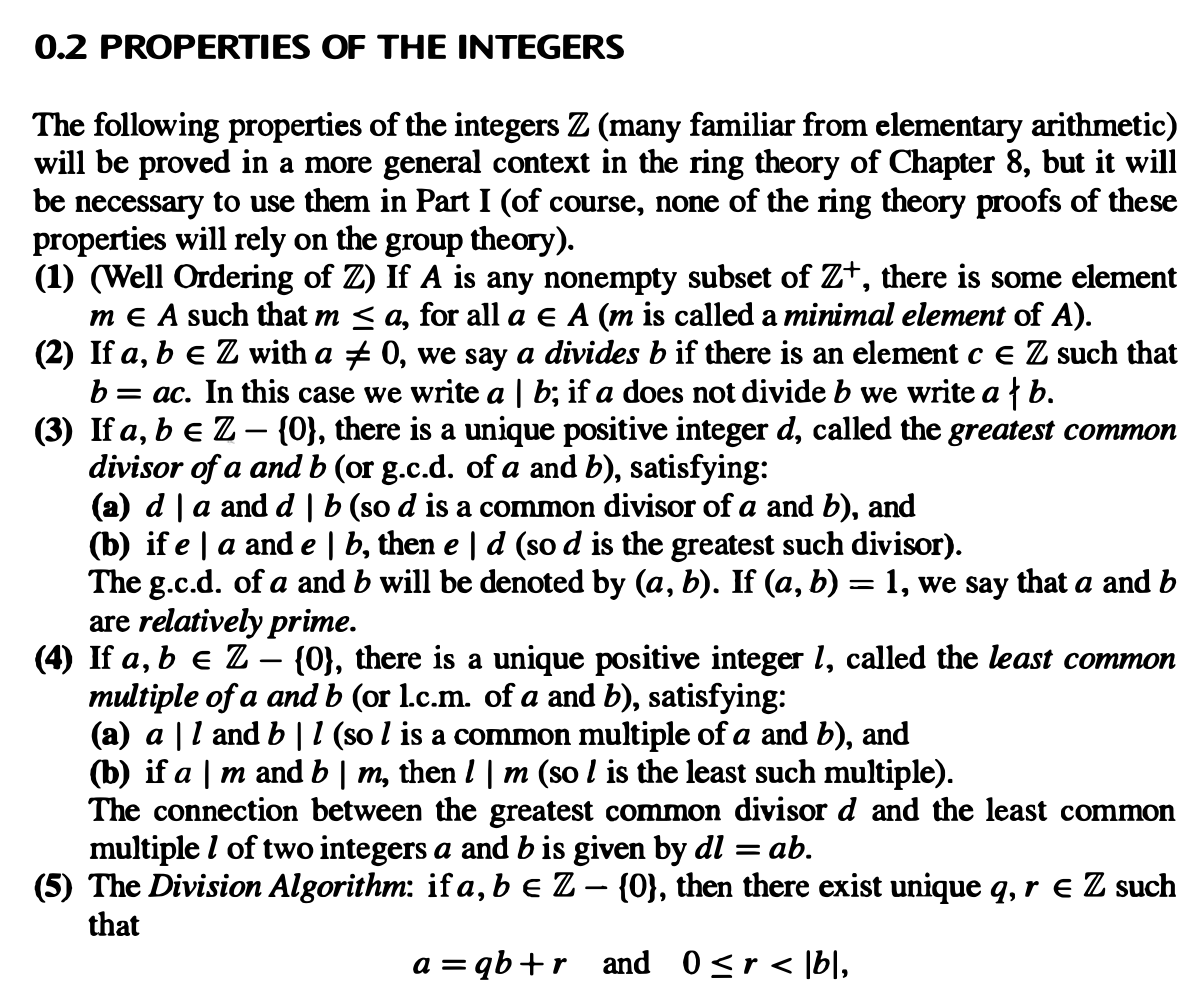
\includegraphics[width=400pt]{img/foundations--set-theory--number-theory-82fa.png}
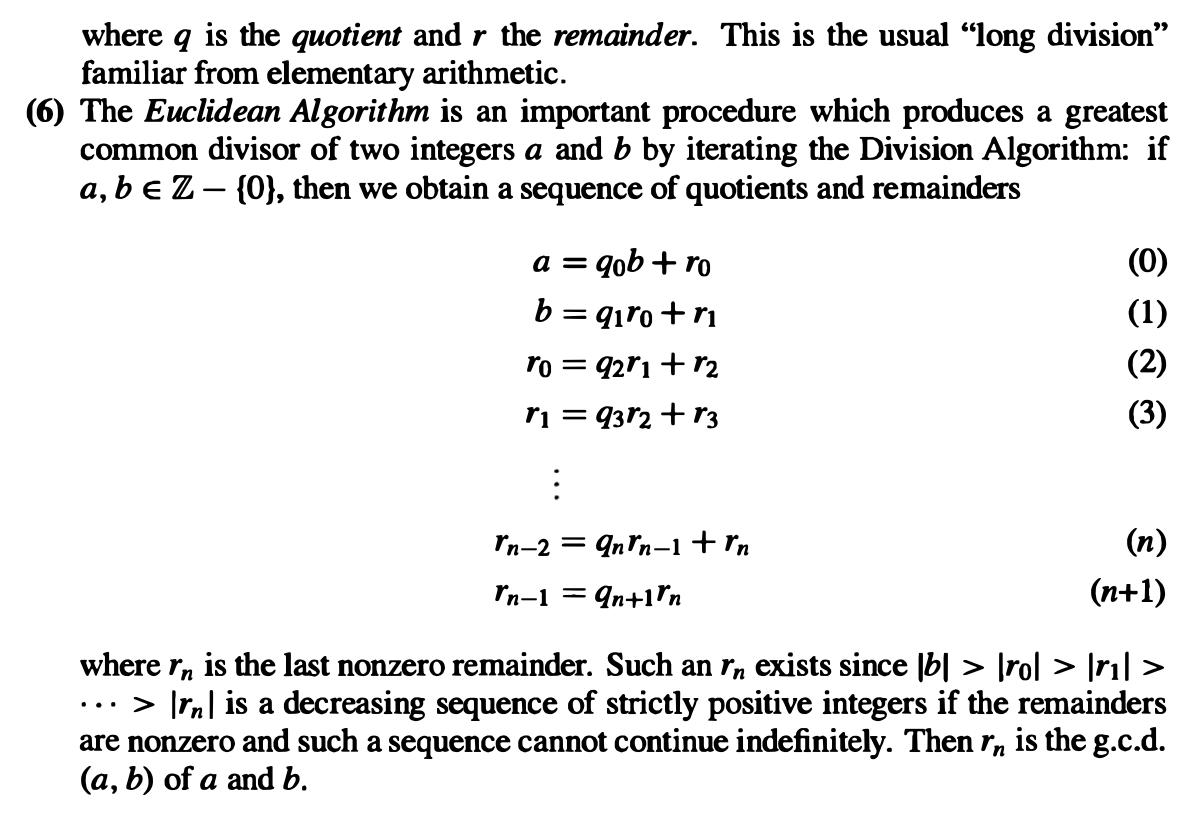
\includegraphics[width=400pt]{img/foundations--set-theory--number-theory-179a.png}
\end{mdframed}
